\chapter{Użyte narzędzia i technologie}\label{chap:technologie}

\section{Zbiór danych}\label{sec:zbior_danych}

\subsection{RedDots}

W pracy wykorzystano zbiór \techname{RedDots}\cite{theReddotsDataCollection}.
Jest to zbiór nagrań głosowych przeznaczony do problemu weryfikacji mówcy.
Jest dostosowany do problemu weryfikacji zależnej od tekstu, gdyż transkrypcja każdej wypowiedzi jest znana,
a mówcy wypowiadają w nim wielokrotnie zdania o tej samej treści. Zbiór został zebrany od ochotników z całego
świata przez Internet, co sprawia, że choć treści wypowiedzi są po angielsku, to mówcy wypowiadają słowa
z różnym akcentem. Nagrania były tworzone w niekontrolowanych warunkach i często są zakłócone.
Wśród ochotników znalazło się 49 mężczyzn i 13 kobiet z 21 krajów.

Gromadzenie danych przebiegało w cotygodniowych sesjach. Autorzy mieli plan zebrać po 52 sesji od każdego uczestnika,
czyli zbierać je przez cały rok, ale w praktyce liczba sesji na mówcę jest bardzo różna. Łącznie przeprowadzono
473 sesji mężczyzn i 99 sesji kobiet, gromadząc 15306 nagrań. W każdej sesji uczestnik miał za zadanie nagrać 24 wypowiedzi.

\begin{itemize}
    \item 10 wypowiedzi miało stałą treść dla wszystkich uczestników i we wszystkich sesjach. Stanowią one podstawę
        pierwszego zadania testowego zdefiniowanego przez twórców. Ich treść to zdania o identyfikatorach $31-40$
        z innego zbioru \shortcut{TIMIT}.
    \item 10 wypowiedzi miało stałą treść we wszystkich sesjach, lecz unikalną dla każdego uczestnika. To znaczy
        każdemu uczestnikowi przydzielono na stałe oddzielny zestaw 10 zdań. Nagrania te są podstawą drugiego zadania.
    \item 2 wypowiedzi o treści nie zmieniającej się między sesjami, lecz wybranej przez uczestnika. Powoduje
        to w porównaniu z poprzednim punktem ryzyko, iż użytkownik wybierze krótkie hasło. Do tego niektórzy
        użytkownicy wybierali zdania w innym języki niż angielski. Pozwala to zbadać efekty pozostawienia wyboru hasła
        użytkownikom i jest przedmiotem trzeciego zadani.
    \item 2 wypowiedzi o treści unikalnej w całym zbiorze. Na ich treść składają się wycinki Wikipedii. Są wykorzystywane
        w czwartym zadaniu, które sprawdza skuteczność systemu na nagraniach o niezarejestrowanej wcześniej treści.
\end{itemize}

Wszystkie nagrania są w nieskompresowanym formacie \shortcut{pcm}, który oznacza, że wartości kolejnych próbek w czasie
są zapisane jedna po drugiej. Częstotliwość próbkowania nagrań to $16$kHz. Do tego zbiór zawiera plik z transkrypcjami
wszystkich wypowiedzi.

Poza tym są pliki z definicjami czterech problemów. Do każdego zadania zdefiniowany został zestaw nagrań rejestracyjnych
(\foreign{enrollment}) i zestaw nagrań weryfikacyjnych. (\foreign{trial}) Zadania te zostały wstępnie przedstawione
w opisie jakie 24 zdania wchodziły w skład sesji.

\begin{enumerate}
    \item Wszyscy mówcy wypowiadają te same 10 zdań. Trzy nagrania na zdanie na osobę przeznaczone są do zapisów. W testach
        są pozostałe nagrania. Każde jest wielokrotnie podawane do systemu w celu weryfikacji czy jest na nim oczekiwany mówca
        i zdanie. Dla każdego nagrania sprawdzane są wszystkie kombinacje znanych mówców i zdań z tej części. Do tego niektórzy
        mówcy nie są obecni w zbiorze rejestracyjnym i występują wyłącznie w zbiorze testowym. Stanowią oni test jak system
        radzi sobie przy otwartym zbiorze osób.
    \item Wszyscy mówcy wypowiadają po 10 zdań, każdy mówca ma swój unikalny zestaw. Podobnie jak powyżej, w zbiorze
        rejestracyjnym są po trzy nagrania na osobę na zdanie. Reszta nagrań służy do testów i niektórzy
        mówcy w testach nie występują w zbiorze rejestracyjnym.
        Jako że treść jest wyłączna dla użytkowników, to w przypadku, gdy mówca się nie zgadza, treść też się nie zgadza.
    \item Wszyscy mówcy wypowiadają po 2 zdania, każdy mówca ma unikalny zestaw. Mówcy sami decydują o treści.
        Przypadek podobny do poprzedniego, lecz wypowiedzi jest mniej i zdarzają się wypowiedzi w innych językach.
    \item
        \begin{enumerate}
            \item Wariant niezależny od tekstu. Zestaw rejestracyjny zawiera po sześć nagrań na osobę o unikalnej treści.
                Zestaw testowy zawiera nagrania, również o unikalnej treści.
            \item Wariant zależny od tekstu. Zestaw rejestracyjny zawiera nagrania z części 1-3. Zestaw testowy również
                zawiera nagrania z poprzednich części oraz dodatkowo nagrania z treścią unikalną w całym zbiorze.
        \end{enumerate}
\end{enumerate}

W przejrzanych pracach zwykle zadania 2 i 3 były ignorowane. Możliwe, że budzą mniejsze zainteresowanie przez fakt,
że różni mówcy zawsze różnią się treścią nagrania. Czyni to te części prostszymi, niż pozostałe dwie.
Dodatkowo nagrań w 3 części jest mniej.
Sprawdzenie jak system działa w sytuacji, gdy ktoś podszywa się pod mówcę i zna jego hasło jest bardzo
ważne w praktycznych zastosowaniach.  Do tego w niektórych pracach ignorowane
były nagrania kobiet, gdyż jest ich kilkakrotnie mniej niż nagrań mężczyzn.
Wszystkie testy uwzględniały część 1 i w większości uwzględniany był wariant części 4.

Zbiór został sporządzony na potrzeby konkursu w 2016 roku. Teraz jest dostępny za darmo pod warunkiem
ograniczenia wykorzystania do celów naukowych. Jest warty uwagi, gdyż trudno znaleźć
zbiór dostosowany do problemu weryfikacji zależnej od tekstu, który byłby publicznie dostępny i darmowy.
Istnieje na przykład zbiór \shortcut{YOHO} oraz zbiór \shortcut{RSR2015}, które
zawierają więcej danych zebranych w lepszych warunkach, lecz wymagają opłaty. Tym niemniej warto
o nich pamiętać.

\subsection{CMUDict}

\techname{CMUDict} to zbiór zawierający zapisy fonetyczne ponad 134000 angielskich słów. Rozróżnione
jest w nim 39 fonemów typowych dla angielskiego. Do tego w samogłoskach wyróżniony jest akcent.
Słowa mogą mieć więcej niż jeden zapis fonetyczny.

Zbiór został wykorzystany do zamiany transkrypcji z \techname{RedDots} na ciągi fonemów. Stała
za tym taka idea, że fonemy będą stanowić lepsze klasy w systemach rozpoznawania mówcy, jak
\shortcut{HMM-GMM}, niż litery, którym mogą w angielskim odpowiadać przeróżne fonemy.
Niestety niektóre wypowiedzi z części trzeciej, wybrane przez użytkowników, były w innych językach
i dla nich operacja zawiodła. Dlatego w systemach, które bazują na fonetycznych transkrypcjach,
są one odrzucane. Nie jest to problemem jeżeli zupełnie zignoruje się trzeci problem.

\section{Sprzęt}\label{sec:sprzet}

Utworzone w ramach pracy programy tworzono i wykonywano na maszynie udostępnionej
w Centrum Technologii Informatycznych Politechniki Łódzkiej. $64$GB pamięci i $40$ rdzeniowy
procesor mocno przyśpieszył pracę oraz umożliwił załadowanie całego zbioru do pamięci.
Praca nie wymaga jednak żadnych niestandardowych urządzeń lub warunków, jej odtworzenie
jest możliwe na zwykłym komputerze.

\section{Technologie}\label{sec:technologie}

\subsection{Język programowania}

Programy utworzone na potrzeby pracy stworzono w języku \techname{Python}. Wybrano go
ze względu na to, iż zdominował popularnością inne języki w dziedzinie przetwarzanie danych.
Wiąże się to z tym, iż istnieje dużo dojrzałych bibliotek, takich jak \techname{scikit-learn}
oraz \techname{TensorFlow}, zawierających implementacje metod, których wykorzystanie jest w planach.
Poza tym bezproblemowo integruje się środowiskiem \techname{Jupyter}, które jest bardzo wygodne przy
zdalnej pracy na klastrze. Umożliwia ono pracę interaktywną, co jest cenne, gdy zachodzi
potrzeba przetestowania wielu rozwiązań i reagowania na wyniki.

\subsection{Biblioteki}

\begin{figure}[H]
    \centering
    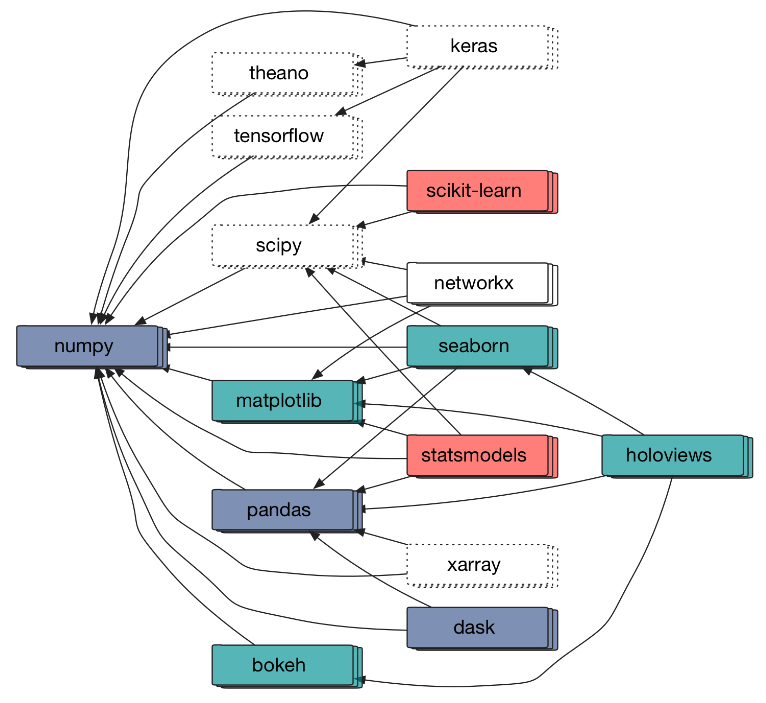
\includegraphics[width=0.6\textwidth]{images/3_3_ecosystem}
    \caption{Ekosystem narzędzi Pythonowych przedstawiony na prezentacji z PyData Warsaw 2017\cite{thePythonEcosystem}}
    \label{fig:3_3_ecosystem}
\end{figure}

Program wykorzystuje popularny \foreign{stack} związany z językiem \techname{Python} składający się z:

\begin{itemize}
    \item \techname{numpy} dostarczający wydajną i uniwersalną implementację macierzy wielowymiarowej i operacji na niej.
        Inne pakiety zależą od tej biblioteki i wykorzystują macierze w swojej implementacji.
    \item \techname{pandas} przede wszystkim udostępnia \foreign{DataFrame}, to znaczy obiekt do przechowywania i analizowania danych tabelarycznych, przypominający w funkcji arkusz kalkulacyjny. W porównaniu z macierzami z \techname{numpy}, \foreign{DataFrame} mogą składać się z kolumn różnych typów i o różnej semantyce. Przy operowaniu na nich często zachodzi potrzeba selekcji, grupowania bądź agregowania, liczenia statystyk opisowych wybranych kolumn.
    \item \techname{scipy} operuje na macierzach \techname{numpy} i dostarcza wiele algorytmów numerycznych, optymalizacyjnych, z algebry liniowej, statystycznych, itd. W tej pracy wykorzystano przede wszystkich moduł z metodami przetwarzania sygnałów.
    \item \techname{scikit-learn} zawiera algorytmy uczenia maszynowego. W pracy przydatna była przede wszystkim implementacja mikstur gaussowskich oraz obliczenia krzywej \shortcut{ROC}.
    \item \techname{matplotlib} pozwala na generowanie statycznych wizualizacji np. spektrogramów, krzywych \shortcut{ROC}. Z jej pomocą wygenerowane zostały także ilustracje konceptów z teorii przetwarzania mowy zaprezentowane w rozdziale \ref{chap:teoria}. Warto wspomnieć, że niektóre z tych ilustracji zostały wygenerowane z użyciem \techname{bokeh} i \techname{holoviews}.
    \item \techname{pickle} uniwersalna biblioteka do serializacji danych. Wykorzystana do zachowania dopasowanych modeli i wyników.
\end{itemize}

Jeśli chodzi o przetwarzanie dźwięku, to wykorzystany został pakiet \techname{python-speech-features}
do obliczenia \shortcut{MFCC} oraz cech delta i delta delta dla nagrań ze zbioru \techname{RedDots}.
Przed przetworzeniem cech używany jest również pakiet \techname{webrtcvad} do przeprowadzenia
\foreign{voice activity detection}, tzn. wykrycia ramek o niskiej energii.  Znalezione ramki z początku i końca są usuwane.

Przy pracach nad ukrytymi modelami Markowa wypróbowane zostały pakiety \techname{hmmlearn} i \techname{pomegranate}.
Niestety sprawiały wiele problemów numerycznych podczas dopasowywania modelu do nagrań. Ostatecznie zrezygnowano z nic
i zastąpiono własną implementacją.

W pracy użyty został również \techname{TensorFlow}. Biblioteka ta dostarcza
implementacji tensora - pozornie macierzy wielowymiarowej jak z \techname{numpy}. Jest jednak
dostosowana do potrzeb implementacji algorytmów uczenia maszynowego. Stosuje model opóźnionej
ewaluacji, podobnie jak \techname{Spark} lub \techname{dask}. To znaczy, że
osobno definiuje się w niej operacje do wykonanie przez zbudowanie grafu i osobno przekazuje go do interpretacji.
Ten sposób wykonania umożliwia dokonanie optymalizacji po zdefiniowaniu obliczeń i przed wykonaniem oraz
obchodzi się tym samym wadę Pythona - relatywnie powolne wykonywanie kodu.
\techname{Tensorflow} zawiera komponenty potrzebne do zdefiniowania grafu, w tym wysokopoziomowe
z pakietu \techname{tf.estimator}. Umożliwia automatyczne obliczanie pochodnych na potrzeby wstecznej propagacji.
Pozwala na wykonywanie operacji na \shortcut{GPU} oraz rozproszenie obliczeń.

W pracy użycie \techname{TensorFlowa} jest jednak ograniczone, gdyż w jej ramach nie jest trenowana żadna
sieć neuronowa. Wykorzystany został gotowy model stworzony przez organizację \techname{Mozilla} w oparciu o
pracę \techname{DeepSpeech}\cite{deepSpeechScaling}, opisującą komercyjny model do rozpoznawania mowy stworzony
przez \techname{Baidu}. Ten model jest wczytywany w sesji \techname{TensorFlowa} i używany do dopasowania
ramek do klas.

\subsection{Narzędzia}

W pracy wykorzystany został \techname{Docker}. Uruchamiany jest w nim obraz \\ \techname{tensorflow/tensorflow:1.4.0-gpu-py3},
z przygotowanym środowiskiem z \techname{TensorFlowem}. Umożliwia to szybką instalację tego pakietu, która ogólnie nie
jest trywialna. W kontenerze uruchamiany jest serwer \techname{Jupyter} i z jego wykorzystaniem przebiegła większość prac.

\techname{Jupyter} stanowi rozwinięcie starszych narzędzi programowania interaktywnego jak \techname{IPython} czy zwykły \techname{Pythonowy} interpreter. W sesjach interaktywnych występuje taki problem, że instrukcje trzeba wprowadzać linijka po linijce, a wpisany kod jest zapisywany w ograniczonej historii. Przeciwieństwem sesji są skrypty, które pozwalają wygodnie manipulować
kodem oraz są trwałe i powtarzalne, lecz zupełnie nieinteraktywne i po każdej zmianie wymagają ponownego wykonania.
\techname{Jupyter} łączy dobre strony obu podejść i pozwala tworzyć skrypty, które można blokami wykonywać
w interaktywnej sesji, tzw. notesy. (\foreign{notebook}, format \techname{ipynb})

\techname{Jupyter} działa jako serwer \shortcut{HTTP} i dostarcza przeglądarkowe środowisko do edycji kodu. Jest ono
ubogie w funkcje, przynajmniej w porównaniu z rozwiniętymi środowiskami programistycznymi. Fakt, że
program działa jako serwer ma taką zaletę, iż można go uruchomić zdalnie na komputerze dysponującym duże zasoby
obliczeniowe oraz bezpośredni dostęp do danych, a następnie pracować na nim zdalnie.

Dużym atutem jest wsparcie dla bibliotek jak \techname{pandas}, \techname{matplotlib} czy \techname{bokeh}.
\foreign{DataFrame} są automatycznie wyświetlane jako tabele, a generowane wizualizacje są bezpośrednio wyświetlane
między blokami notesu. Jest też możliwość tworzenia interaktywnych elementów jak przyciski czy pola tekstowe i
w reakcji na zmiany ich stanu wykonywać kod w interaktywnej sesji.

Poza tym warto wspomnieć, że wykorzystano \techname{gita} do wersjonowania pracy, zarówno \foreign{notebooków}, pakietów jak i tekstu tego dokumentu. Do zarządzania pakietów wykorzystano \techname{pip}, ale być może lepszym wyborem są nowsze narzędzia jak \techname{conda} lub \techname{pipenv}.

